\section{Manual de usuario aplicativo GEE}

En el contexto presente, el manual de usuario del aplicativo GEE se presenta como una guía integral para la utilización efectiva de la herramienta. Este manual está diseñado para facilitar la comprensión y el uso del aplicativo, proporcionando instrucciones claras y concisas sobre su funcionamiento.

El aplicativo GEE, desarrollado en Google Earth Engine, permite la visualización y análisis de datos geoespaciales relacionados con la temperatura superficial del mar (TSM) y su correlación con el índice de vegetación de diferencia normalizada (NDVI). A través de este manual, los usuarios podrán familiarizarse con las funcionalidades del aplicativo, así como con los pasos necesarios para llevar a cabo un análisis efectivo de los datos disponibles.

\subsection{Descripción de la interfaz}

La interfaz del aplicativo GEE está diseñada para ser intuitiva y fácil de usar. En $[1]$, se presenta el mapa espacio donde los usuarios pueden visualizar el área de muestra de cobertura agrícola permanente, luego en $[2]$ se muestra el panel de opciones se detalla primero la entidad que presenta la herramienta seguido de información acerca del aplicativo. A continuación de ello se muestran los botones selectores de zona de estudio.

\begin{figure}[ht]
  \centering
  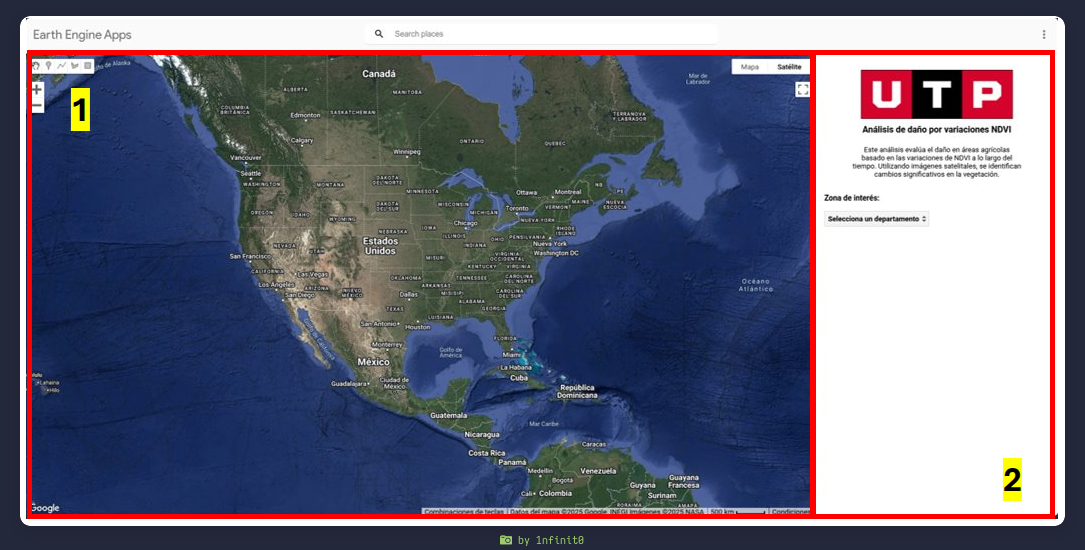
\includegraphics[width=\textwidth, trim=20px 25px 20px 20px, clip]{assets/canvas.png}
  \caption{Primera pantalla del aplicativo GEE.}
  \label{fig:canvas}
\end{figure}

\subsection{Uso del aplicativo}

El aplicativo GEE permite a los usuarios seleccionar un distrito dada una lista de departamentos y provincias. $[1]$.

Una vez seleccionada la zona de estudio, el aplicativo solicitará escoger un mes en específico, esta información servirá para poder realizar las operaciones descritas por los algoritmos mencionados. $[2]$.

\begin{figure}[ht]
  \centering
  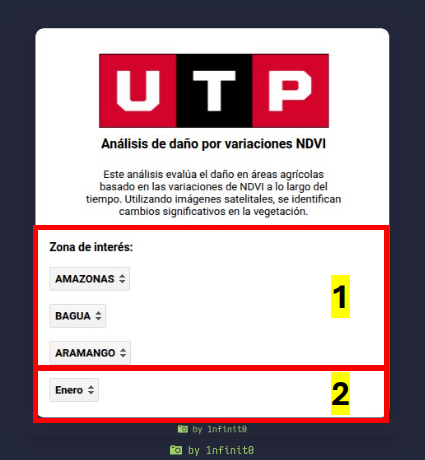
\includegraphics[width=7cm, trim=37px 38px 38px 50px, clip]{assets/panel.png}
  \caption{Panel de selección de área de interés}
  \label{fig:panel}
\end{figure}

\subsection{Interpretación de gráficos}

Una vez seleccionada la zona de estudio y el mes, el aplicativo generará 4 gráficos:

En $[1]$ se muestra el monitoreo del ICEN mensual en los últimos 12 registros que se hayan actualizado en la plataforma del IGP, esto con la finalidad de poder realizar un análisis de la tendencia del índice de calor en el área seleccionada. En $[2]$ se muestra el monitoreo la anomalía de TSM mensual en los últimos 12 meses desde el momento de consulta, esta información proporcionada por el sensor MODIS-AQUA.

\begin{figure}[ht]
  \centering
  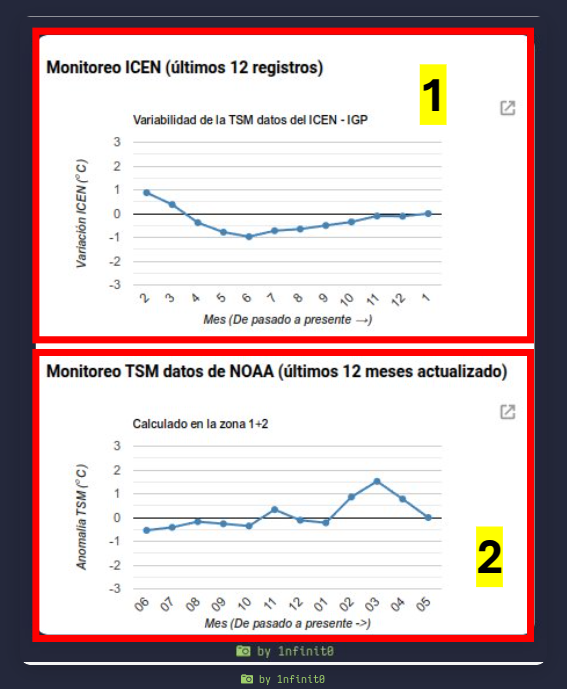
\includegraphics[width=7cm, trim=37px 48px 38px 32px, clip]{assets/grafico1.png}
  \caption{Gráficos de monitoreo de anomalía TSM}
  \label{fig:tsm}
\end{figure}

\newpage

En $[3]$ se muestra el monitoreo del NDVI del mes seleecionado y se compara con los niveles del mismo mes en los últimos 15 años, esto con la finalidad de poder realizar un análisis de la tendencia en comparación con los ciclos en los cuales ocurren estos fenómenos. Finalmente, en $[4]$ se muestra la correlación de estos valores en el área seleccionada, lo que pretende brindar una idea del nivel de vulnerabilidad de la zona de estudio ante el fenómeno climático.

\begin{figure}[ht]
  \centering
  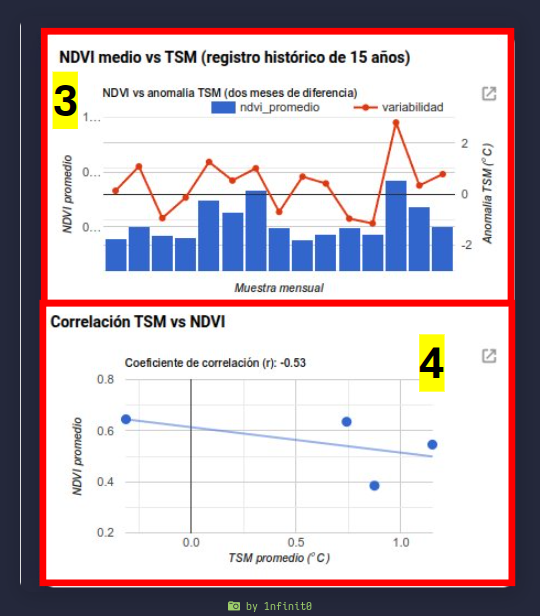
\includegraphics[width=8cm, trim=37px 29px 25px 25px, clip]{assets/correlacion.png}
  \caption{Gráficos de NDVI histórico y correlación}
  \label{fig:correlación}
\end{figure}